\documentclass{article}

% if you need to pass options to natbib, use, e.g.:
%     \PassOptionsToPackage{numbers, compress}{natbib}
% before loading neurips_2019

% ready for submission
% \usepackage{neurips_2019}

% to compile a preprint version, e.g., for submission to arXiv, add add the
% [preprint] option:
%     \usepackage[preprint]{neurips_2019}

% to compile a camera-ready version, add the [final] option, e.g.:
\usepackage[final]{neurips_2019}

% to avoid loading the natbib package, add option nonatbib:
%     \usepackage[nonatbib]{neurips_2019}

\usepackage[utf8]{inputenc} % allow utf-8 input
\usepackage[T1]{fontenc}    % use 8-bit T1 fonts
\usepackage{hyperref}       % hyperlinks
\usepackage{url}            % simple URL typesetting
\usepackage{booktabs}       % professional-quality tables
\usepackage{amsmath}
\usepackage{amsfonts}       % blackboard math symbols
\usepackage{nicefrac}       % compact symbols for 1/2, etc.
\usepackage{microtype}      % microtypography
\usepackage{graphicx}
\newcommand{\indep}{\rotatebox[origin=c]{90}{$\models$}}

\title{1RT705: Group Martin Hellkvist (1 members)}

% The \author macro works with any number of authors. There are two commands
% used to separate the names and addresses of multiple authors: \And and \AND.
%
% Using \And between authors leaves it to LaTeX to determine where to break the
% lines. Using \AND forces a line break at that point. So, if LaTeX puts 3 of 4
% authors names on the first line, and the last on the second line, try using
% \AND instead of \And before the third author name.

%\author{%
%	David S.~Hippocampus\thanks{Use footnote for providing further information
%		about author (webpage, alternative address)---\emph{not} for acknowledging
%		funding agencies.} \\
%	Department of Computer Science\\
%	Cranberry-Lemon University\\
%	Pittsburgh, PA 15213 \\
%	\texttt{hippo@cs.cranberry-lemon.edu} \\
	% examples of more authors
	% \And
	% Coauthor \\
	% Affiliation \\
	% Address \\
	% \texttt{email} \\
	% \AND
	% Coauthor \\
	% Affiliation \\
	% Address \\
	% \texttt{email} \\
	% \And
	% Coauthor \\
	% Affiliation \\
	% Address \\
	% \texttt{email} \\
	% \And
	% Coauthor \\
	% Affiliation \\
	% Address \\
	% \texttt{email} \\
%}

\begin{document}
	
	\maketitle
%	
%	\begin{abstract}
%		The abstract paragraph should be indented \nicefrac{1}{2}~inch (3~picas) on
%		both the left- and right-hand margins. Use 10~point type, with a vertical
%		spacing (leading) of 11~points.  The word \textbf{Abstract} must be centered,
%		bold, and in point size 12. Two line spaces precede the abstract. The abstract
%		must be limited to one paragraph.
%	\end{abstract}
	
	\section{Outline}
	The layout of this report is designed to answer the questions Q1 through Q10 in ascending order. The title of each section is named so it describes what questions it will give answers to.
	\section{Modeling (Q1-Q3)}
	\label{sec:modeling}
	The \textit{TrueSkill} Bayesian model for one match can be formulated as
	
	\begin{subequations}
	\begin{align}\label{eqn:model}
	p(s_1) &= \mathcal{N}(s_1; \mu_1, \sigma_1^2),\\
	p(s_2) &= \mathcal{N}(s_2; \mu_2, \sigma_2^2),\\
	p(t|s_1, s_2) &= \mathcal{N}(t; s_1-s_2, \sigma_t^2),\\
	y &= \text{sign}(t),
	\end{align}
	\end{subequations}
	where $ \{\mu_1,\mu_2,\sigma_1,\sigma_2,\sigma_t\} $ are the hyperparameters to set. Microsoft states\footnote{\url{https://www.microsoft.com/en-us/research/project/trueskill-ranking-system/} (accessed: 25 Sep. 2019)} that in their implementation of the \textit{TrueSkill} model, the default value for new players is $ \mu=25, \sigma=8.3333 $ and that the \textit{TrueSkill} value for that player is $25-3\cdot8.3333=0$, being the conservative estimate of the player's skill. 
	
	Gathering $ s_1 $ and $ s_2 $ as $s = (s_1, s_2)$, the conditional distribution of the skills $p(s_1, s_2|t,y)$ can be computed using Corollary 1 from the lectures of the course:
	
	\begin{subequations}
	\begin{align}
		p(s | t, y) &= p(s | t) = \mathcal{N}\Big( s;~\mu_{s|t},\,\Sigma_{s|t} \Big),\\
		\mu_{s|t} &= \Sigma_{s|t}\Big(\Sigma_s^{-1} \mu_s + M^T\Sigma_{t|s}^{-1}t\Big),\\
		\Sigma_{s|t} &= \Big( \Sigma_s^{-1} + M^T\Sigma_{t|s}^{-1}M \Big)^{-1},
	\end{align}
	\end{subequations}
	where the covariance matrix for $t$ given $s$ is just $\Sigma_{t|s}=\sigma_t^2$ from the model \eqref{eqn:model}, the matrix $M$ is $[1, -1]$ so that $M^Ts = s_1 - s_2$, the covariance matrix for s is $\Sigma_s = \begin{bmatrix}
	\sigma_1^2 & 0\\ 0 & \sigma_2 \end{bmatrix}$ and the mean vector for s is $\mu_s = [\mu_1, \mu_2]^T$.
	
	The full conditional distribution for the outcome $t$ becomes a truncated normal distribution, due to the information from $y$ that indicates the sign of the variable $t$:
	\begin{align}
	p(t|s_1, s_2, y) = \mathcal{TN}(t;~s_1-s_2, \sigma_t^2, y),
	\end{align}
	where we let the notation $\mathcal{TN}(x;~\mu, \sigma^2, a)$ be the normal distribution $\mathcal{N}(x;~\mu, \sigma^2)$ while the pdf is zero for $ x<0 $ if $ y=1 $, or zero for $ x>0 $ if $ y=-1 $.
	
	The marginal probability of $ y=1 $ is computed by marginalizing the joint distribution that can be formulated from the Bayesian network in figure \ref{fig:bayes_n}.
	
	\begin{align}
	\begin{split}
	p(y=1) 	&= \int_{s_1}\int_{s_2}\int_t p(s_1, s_2, t, y=1)\,ds_1\,ds_2\,dt=\\
			&= \int_{s_1}p(s_1)\int_{s_2}p(s_2)\int_t p(t|s_1,s_2)p(y=1|t)\,dt\,ds_2\,ds_1\\
			&= \int_{s_1}p(s_1)\int_{s_2}p(s_2)\int_0^\infty p(t|s_1,s_2)\,dt\,ds_2\,ds_1\\
			&= \int_{s_1}p(s_1)\int_{s_2}p(s_2) (1 - D(t=0|s_1,s_2))\,ds_2\,ds_1\\
			&= (1-D(t=0|s_1,s_2))\int_{s_1}p(s_1)ds_1\int_{s_2}p(s_2)ds_2\\
			&= (1-D(t=0|s_1,s_2)) = (1 - \dfrac{1}{2}(1+\text{erf}\Big(\dfrac{0-(s_1-s_2)}{\sigma_t\sqrt{2}}\Big)))\\
			&= \dfrac{1}{2}\Big(1 - \text{erf}\Big(\dfrac{s_2-s_1}{\sigma_t\sqrt{2}}\Big)\Big),
	\end{split}
	\end{align}
	where $ D(t|s_1,s_2) = \frac{1}{2}(1+\text{erf}(\frac{t-(s_1-s_2)}{\sigma_t\sqrt{2}}))$ is the cumulative distribution function of $p(t|s_1,s_2)$ \cite{MATHWORLDWOLFRAM.COM}.
	
	A Bayesian network of the model \eqref{eqn:model} is presented in figure \ref{fig:bayes_n}, from which we together with rules of independence in Bayesian networks [\cite{asdf1337}] can observe two conditionally independent sets of variables as:
	
	\begin{align}
		s_1 \,\indep \, s_2 ~|~ \emptyset, \\
		s_1 \,\indep \, y ~|~ t.
	\end{align}
	
	\begin{figure}[t]
		\centering
		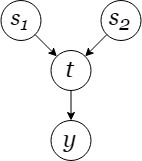
\includegraphics[width=0.2\linewidth]{bayes4}
		\caption{A Bayesian network of the model in \eqref{eqn:model}.}
		\label{fig:bayes_n}
	\end{figure}
	
	\section{Gibbs Sampling (Q4)}
	The initialization of the Gibbs sampler in this exercise consists of choosing a value for $t_0$. Figure \ref{fig:q_4_1} illustrates the propagation of the samples over the first 200 iterations of the Gibbs sampler for $t_0=100$ (i.e., player 1 wins by a huge margin -- in terms of football) and the other parameters set as discussed in section \ref{sec:modeling} and assuming $y=1$. From this plot, a burn-in of 50 samples seems reasonable, and it showed consistency over independent simulations.
	\begin{figure}[t]
		\centering
		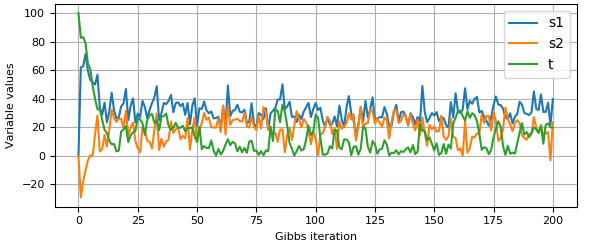
\includegraphics[width=.7\linewidth]{q_4_1}
		\caption{Samples of the variables $ s_1,s_2,t $ for 200 Gibbs sampler iterations.}  
		\label{fig:q_4_1}
	\end{figure}

	The histograms in figure \ref{fig:q_4_2} illustrates that the choice of $K=350$ samples after the burn-in period of $50$ samples is almost as precise as $K=1000$, while running in less than half that simulation's time. For the following experiments, $K=350$ is used together with the $50$ samples burn-in period.
	
	\begin{figure}[t]
		\centering
		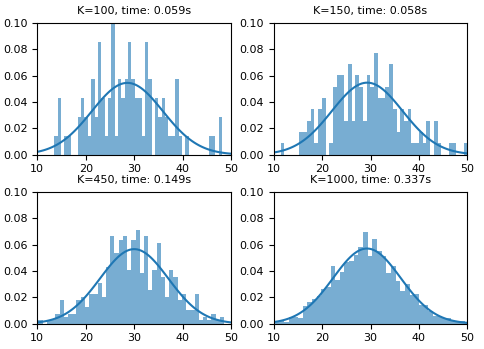
\includegraphics[width=0.7\linewidth]{q_4_2}
		\caption{Histograms of the samples (post burn-in) and the estimated posteriors for different values of $K$. The mean and standard deviation of the posteriors were estimated as the empirical mean and standard deviation of the samples from the Gibbs sampler.}
		\label{fig:q_4_2}
	\end{figure}
	
	
	
	\section{Assumed Density Filtering and Predictions (Q5-Q6)}
	
	
	\begin{table}[t]
		\caption{Mean, variance and conservative estimate of each team's skill after all matches simulated in two different orders.}
		\label{tab:q4}
		\centering
		\begin{tabular}{lrrr|lrrr}
			\toprule
			\multicolumn{4}{c}{Chronological order} & \multicolumn{4}{c}{Reversed chronological order} \\
			\midrule
			Team     		& $ \mu $ & $ \sigma $ & $ \mu - 3\sigma $ & Team & $ \mu $ & $ \sigma $ & $ \mu-3\sigma $\\
			\midrule
		Inter           & 29.03 & 1.55 & 24.39 & Juventus  & 32.09 & 1.43 & 27.81 \\
		Napoli          & 29.66 & 1.82 & 24.20 & Napoli    & 30.10 & 1.31 & 26.19 \\
		Milan           & 28.92 & 1.69 & 23.84 & Inter     & 27.79 & 1.48 & 23.36 \\
		Juventus        & 29.98 & 2.08 & 23.73 & Milan     & 27.24 & 1.56 & 22.54 \\
		Torino          & 28.17 & 1.49 & 23.70 & Roma      & 26.68 & 1.54 & 22.06 \\
		Atalanta        & 28.48 & 1.67 & 23.47 & Atalanta  & 26.41 & 1.47 & 21.99 \\
		Roma            & 27.25 & 1.37 & 23.14 & Lazio     & 25.14 & 1.24 & 21.40 \\
		Sampdoria       & 24.84 & 1.33 & 20.83 & Torino    & 27.60 & 2.16 & 21.12 \\
		Lazio           & 25.77 & 1.66 & 20.80 & Sampdoria & 25.70 & 1.66 & 20.73 \\
		Parma           & 23.54 & 1.09 & 20.27 & Parma     & 23.55 & 1.53 & 18.95 \\
		Bologna         & 24.18 & 1.43 & 19.89 & Spal      & 22.50 & 1.30 & 18.60 \\
		Spal            & 23.97 & 1.43 & 19.66 & Udinese   & 22.54 & 1.35 & 18.51 \\
		Udinese         & 23.72 & 1.48 & 19.27 & Sassuolo  & 23.16 & 1.61 & 18.32 \\
		Empoli          & 23.38 & 1.64 & 18.47 & Genoa     & 22.86 & 1.80 & 17.45 \\
		Genoa           & 23.36 & 1.68 & 18.31 & Cagliari  & 22.24 & 1.66 & 17.26 \\
		Cagliari        & 22.79 & 1.65 & 17.83 & Fiorentina& 22.36 & 1.80 & 16.97 \\
		Fiorentina      & 22.29 & 1.80 & 16.89 & Empoli    & 21.67 & 1.59 & 16.91 \\
		Sassuolo        & 22.40 & 1.92 & 16.64 & Bologna   & 21.90 & 1.93 & 16.12 \\
		Frosinone       & 19.95 & 1.37 & 15.84 & Frosinone & 18.36 & 1.88 & 12.73 \\
		Chievo          & 17.00 & 2.20 & 10.41 & Chievo    & 14.37 & 2.13 &  7.98 \\ \bottomrule
		\end{tabular}
	\end{table}
	
	
	
	\begin{figure}
		\centering
		\fbox{\rule[-.5cm]{0cm}{4cm} \rule[-.5cm]{4cm}{0cm}}
		\caption{Sample figure caption.}
	\end{figure}
	\begin{table}
		\caption{Sample table title}
		\label{sample-table}
		\centering
		\begin{tabular}{lll}
			\toprule
			\multicolumn{2}{c}{Part}                   \\
			\cmidrule(r){1-2}
			Name     & Description     & Size ($\mu$m) \\
			\midrule
			Dendrite & Input terminal  & $\sim$100     \\
			Axon     & Output terminal & $\sim$10      \\
			Soma     & Cell body       & up to $10^6$  \\
			\bottomrule
		\end{tabular}
	\end{table}

	\section*{References}
	
	References follow the acknowledgments. Use unnumbered first-level heading for
	the references. Any choice of citation style is acceptable as long as you are
	consistent. It is permissible to reduce the font size to \verb+small+ (9 point)
	when listing the references. {\bf Remember that you can use more than eight
		pages as long as the additional pages contain \emph{only} cited references.}
	\medskip
	
	\small
	
	[1] Alexander, J.A.\ \& Mozer, M.C.\ (1995) Template-based algorithms for
	connectionist rule extraction. In G.\ Tesauro, D.S.\ Touretzky and T.K.\ Leen
	(eds.), {\it Advances in Neural Information Processing Systems 7},
	pp.\ 609--616. Cambridge, MA: MIT Press.
	
	[2] Bower, J.M.\ \& Beeman, D.\ (1995) {\it The Book of GENESIS: Exploring
		Realistic Neural Models with the GEneral NEural SImulation System.}  New York:
	TELOS/Springer--Verlag.
	
	[3] Hasselmo, M.E., Schnell, E.\ \& Barkai, E.\ (1995) Dynamics of learning and
	recall at excitatory recurrent synapses and cholinergic modulation in rat
	hippocampal region CA3. {\it Journal of Neuroscience} {\bf 15}(7):5249-5262.
	
\end{document}